\documentclass[11pt,a4paper]{article}
\usepackage{xcolor}
\usepackage{listings}
\usepackage{graphicx}
\usepackage{times}
\usepackage{caption}
\usepackage{amsmath,amssymb}
\usepackage{fancyhdr}                                
\usepackage{hyperref}
\usepackage{CJKutf8}
\usepackage{courier}
\pagestyle{fancy}
\lhead{JOS Arm}   
\rhead{Yiru Chen 1400012976}           
\begin{document}
\begin{CJK}{UTF8}{gkai}%gkai  gbsn
 \lstset{
         basicstyle=\footnotesize\ttfamily, % Standardschrift
         %numbers=left,               % Ort der Zeilennummern
         numberstyle=\tiny,          % Stil der Zeilennummern
         %stepnumber=2,               % Abstand zwischen den Zeilennummern
         numbersep=5pt,              % Abstand der Nummern zum Text
         tabsize=2,                  % Groesse von Tabs
         extendedchars=true,         %
         breaklines=true,            % Zeilen werden Umgebrochen
         keywordstyle=\color{red},
            frame=b,         
 keywordstyle=[1]\textbf,    % Stil der Keywords
      keywordstyle=[2]\textbf,    %
        keywordstyle=[3]\textbf,    %
 %        keywordstyle=[4]\textbf,   \sqrt{\sqrt{}} %
         stringstyle=\color{orange}\ttfamily, % Farbe der String
	commentstyle=\color{red!50!green!50!blue!02},
         showspaces=false,           % Leerzeichen anzeigen ?
         showtabs=false,             % Tabs anzeigen ?
         xleftmargin=17pt,
         framexleftmargin=17pt,
         framexrightmargin=5pt,
         framexbottommargin=4pt,
         backgroundcolor=\color{red!120!green!50!blue!02},
         showstringspaces=false      % Leerzeichen in Strings anzeigen ?        
 }
 \lstloadlanguages{% Check Dokumentation for further languages ...
         %[Visual]Basic
         %Pascal
         %C
         C++
         %XML
         %HTML
         %Java
 }
 \lstset{numbers=left, 
numberstyle= \tiny, 
keywordstyle= \color{ blue!70},commentstyle=\color{red!20!green!60!blue!30}, 
frame=shadowbox, 
rulesepcolor= \color{ red!70!green!20!blue!20} 
} 
%\begin{center}
%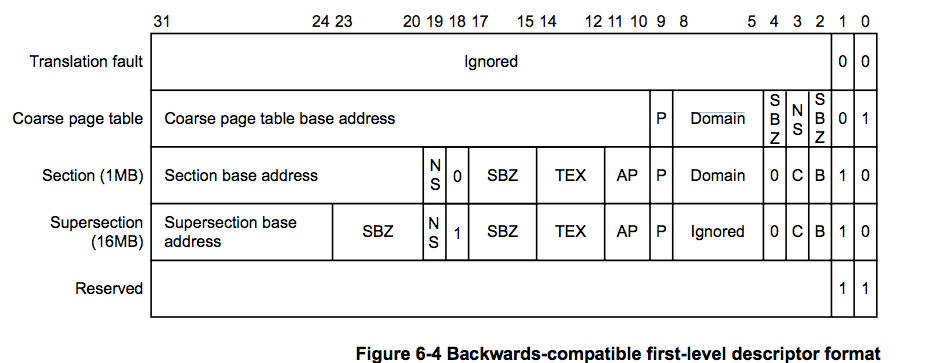
\includegraphics[width=5in]{1.png}
%\end{center}

%\begin{lstlisting}[language=C]
%\end{lstlisting}

\title{\textbf{JOS 2016 JOS ARM移植}}
\author{陈一茹 1400012976}
\date{\today}
\maketitle
\tableofcontents
\newpage

\section{Introduction}
	这次lab是要完成将Intel x86体系结构的JOS移植到ARM平台上。
	
	在这次移植工作,我完成了lab1 和lab2的具体设计和代码实现,这部分将在接下来的报告中详细说明。
	
	首先,要进行移植,首先我们要理解ARM 的体系结构。
	
	\subsection{ARM Introduction}
	ARM架构,过去称作高级精简指令集机器(英语:Advanced RISC Machine,更早称作:Acorn RISC Machine),是一个32位精简指令集(RISC)处理器架构,其广泛地使用在许多嵌入式系统设计。但在其他领域上也有很多作为,由于节能的特点,ARM处理器非常适用于移动通信领域,匹配其主要设计目标为低成本、高性能、低耗电的特性。另一方面,超级计算机消耗大量电能,ARM同样被视作更高效的选择。
	
	至2009年为止,ARM架构处理器占市面上所有32位嵌入式RISC处理器90\%的比例,使它成为占全世界最多数的32位架构之一。ARM处理器可以在很多消费性电子产品上看到,从便携式设备(PDA、移动电话、多媒体播放器、掌上型电子游戏和计算机)到电脑外设(硬盘、桌面型路由器),甚至在导弹的弹载计算机等军用设施中都有他的存在。在此还有一些基于ARM设计的衍申产品,重要产品还包括Marvell的XScale架构和德州仪器的OMAP系列。
	

	\subsection{Experiment Environment}
	我们的目标是将系统跑在Raspberry Pi 2。
	
	树莓派2代的Model B采用Broadcom BCM2836 900MHz的四核SoC,1GB内存,是新一代开拓者,兼容1代B+。但相比之下,树莓派2的性能提升6倍,内存翻了一番。Raspberry Pi 2不仅能跑全系列ARM GNU/Linux发行版,而且支持Snappy Ubuntu Core及Windows 10。但是Broadcom BCM2836的手册是保密的,连原理图都不公开。
	
	由于我们条件所限,我们选用qemu模拟的树莓派2 进行验证测试。qemu是在官网上http://wiki.qemu.org/Main\_Page下载的源代码包,然后编译安装。
	
	从网上查到相关教程,用以下三条指令就可以实现
	
		\begin{lstlisting}
		./configure --target-list=arm-softmmu --prefix=<prefix>
		make 
		make install
		\end{lstlisting}
	
	我们要安装交叉编译器(cross compiler), 因为我是在intel x86的环境下编译arm 的程序,如果我不用交叉编译器,我的机器就不知道我正在跑其他的程序,然后就会遇到不正确的问题。
	这部分是查阅相关文档, 比如 http://wiki.osdev.org/GCC\_Cross-Compiler进行学习完成的。
	
	用以下几个命令,我们可以完成相关的工具的安装,这两个分别是相应的ARM版本下的gcc编译工具链,具体而言就是arm-none-eabi目标平台。
	
	\begin{lstlisting}
	sudo apt-get install gcc-arm-none-eabi
	sudo apt-get install gdb-arm-none-eabi
	\end{lstlisting}
	
	安装完成之后,我就可以开始开发了。
	
\section{Lab1 \& Lab2 Transplant}

	\subsection{JOS on x86 Review}
	首先,我要先回忆一下lab1和lab2 on x86的内容:
	
	\begin{itemize}
		\item BIOS首先初始化
		\item BIOS 将Bootloader加载进内存, 将控制权交给Boot Loader
		\item Boot loader 中代码开始执行,将kernel 读进内存0x100000的地方
		\item 设置好GDT之后,JOS内核首先开始执行的是entry.S,然后调用内核中的i386\_init(),在这个函数中调用cons\_init()进行初始化。JOS中的主要流程都在这个函数中。
		\item 然后调用kern/pmap.c中的mem\_init()进行存储管理的相关设置,进行内存的初始化
		\item 最后monitor()启动命令行,等待用户从终端进行输入。		
	\end{itemize}

	Lab2的任务是实现操作系统的内存管理功能。作为每个软件都要 用到的基本系统资源,内存的管理是操作系统最基本的功能之一。 页存储、虚拟内存等技术广泛应用于现代操作系统中,其也是 Lab2主要实现的功能。

	和大多数嵌入式设备一样, 树莓派2的bootloader是烧在芯片上的,而不是用户定义的(事实上在树莓派上做实验的时候也只是进行了一个ELF替换),因此直接启动内核的方式是合理的。
	
	基于以上内容,我的基本操作系统就不用包括bootloader,只包括bootloader工作完成之后的内核ELF被加载到内存中的工作,(在JOS中是entry.S 开始的),对应的寄存器进行初始化,清零BSS段等一系列的工作。
	
	\subsection{entry.S}
		我实现的entry.S 有三个功能:
		
		\begin{itemize}
			\item 初始化BSS段。
			\item 开启分页模式。
			\item 跳转到高地址,进入init函数。
		\end{itemize}
	
		具体的实现为:
		
		\paragraph{Initialize BSS}
		
		我用了stmia指令进行赋值操作,全局使用一个循环将edata~end间的数据全部清零。
		edata~end区间恰好是bss段,具体可见kernel.ld中的定义。
		\begin{lstlisting}
		// Clear out bss.
		ldr r4, = edata
		ldr r9, = end
		mov r5, #0
		mov r6, #0
		mov r7, #0
		mov r8, #0
		b	check
		
		zero:
			// store multiple at r4.
			stmia r4!, {r5-r8}
		
		// If we are still below bss_end, loop.
		check:
			cmp r4, r9
			blo zero
		\end{lstlisting}
		
		\paragraph{Turn on the MMU}
		这部分需要学习的知识比较多,而且需要了解三个主要的寄存器的用法。
		
		\textbf{两个重要的指令MCR, MRC}
		这两个指令是用来访问CP15寄存器的指令。MCR指令和MRC指令只能在处理器模式为系统模式时执行,在用户模式下执行MCR指令和MRC指令将会触发未定义指令的异常中断。
		
		\begin{itemize}
			\item MCR   ARM寄存器到协处理器寄存器的数据传送。如果协处理器不能成功地执行该操作,将产生未定义的指令异常中断。
			
			指令语法格式
			
			$$MCR\{<cond>\} <p>,<op_1>,<Rd>,<CRn>,<CRm>\{,<op_2>\}  $$
			
			\item MRC   协处理器寄存器到ARM寄存器的数据传送
			
			指令语法格式
			
			$$ MCR\{<cond>\} <p>,<op_1>,<Rd>,<CRn>,<CRm>\{,<op_2>\}$$
			
			其中,$<cond>$为指令执行的条件码。当$<cond>$忽略时指令为无条件执行。
			
		$<op_1>$为协处理器将执行的操作的操作码。对于CP15协处理器来说,$<op_1>$
		永远为0b000,当$<op_1>$不为0b000时,该指令操作结果不可预知。
			
			
			$<Rd>$作为源寄存器的ARM寄存器,其值将被传送到协处理器寄存器中。
			
		$<CRn>$作为目标寄存器的协处理器寄存器,其编号可能是C0,C1,…,C15。
			
		$<CRm>$和$<op_2>$两者组合决定对协处理器寄存器进行所需要的操作,如果没有指定,
		则将为$<CRm>$为C0,$<op_2>$为0,否则可能导致不可预知的结果。
		\end{itemize}
		
		
		\textbf{CP15的寄存器}
		
		CP15 有16个寄存器C0-C15,这里用到是C1,C2, C3。
		
		\begin{itemize}
			\item C1寄存器: Control Register 
				其中最重要的是最后一位:MMU enable:
					0 = MMU disable,
					1 = MMU enable
			\item C2寄存器:Translation Table Base(TTB) Register
				C2寄存器类似于x86的cr3寄存器,用来存储第一级页表的基地址。 
				由于ARM的一级页表有4096项,共占用16KB(后面会详细说明),
				基地址要求是16KB对齐的。
			\item C3寄存器:Domain Access Control Register
				C3寄存器是域访问控制寄存器。域(domain)是x86中没有的概念。
				在ARM中一共存在16个域(0~15),每个虚拟页都从属于某一个域。
				一个域有4种状态,分别为:
					00:该域下的所有内存都不可访问
					01(Client):对该域下的内存访问进行权限检查
					10:Reserved,暂时未定义。
					11(Manager):对该域下的内存访问不进行权限检查
				C3是32位寄存器,2字节分为一组共16组,恰好保存16个域的状态。
		\end{itemize}
		在我的代码中,首先设置C2寄存器,将页表基地址设为entry\_pgdir;
		再设置C3寄存器,将所有域都设置为Manager;
		最后通过设置C1寄存器的enable位开启MMU。
		
		\begin{lstlisting}
		// Turn on the MMU
		ldr r0, =(entry_pgdir - KERNBASE)
		mcr p15, 0, r0, c2, c0, 0
		
		mov r0, #0xFFFFFFFF
		mcr p15, 0, r0, c3, c0, 0
		
		mrc p15, 0, r0, c1, c0, 0
		orr r0, r0, #0x1
		mcr p15, 0, r0, c1, c0, 0
		\end{lstlisting}
		
		\paragraph{Enter the C code}
		和x86类似,我们要先从低地址跳转到高地址,然后设置内核栈,最后调用arm\_init()进入C语言中继续执行。
			\begin{lstlisting}
			//Jump up above KERNBASE before entering C code
			ldr lr, =relocated
			bx lr
		relocated:
			ldr sp, =bootstacktop  // Setup the stack.
			bl arm_init
		
		.data
			// boot stack
			.p2align        20         // force page alignment
			.globl          bootstack
		bootstack:
			.space          0x8000
			.globl          bootstacktop
		bootstacktop:
		\end{lstlisting}
	
	\subsection{init.c}
	在这里我实现了和jos中i386\_init()对应的arm\_init(),对于Lab1和Lab2的移植,我实现了3个功能:
	\begin{enumerate}
		\item 初始化console的输入输出
		\item 初始化页表管理
		\item 进入monitor
	\end{enumerate}
	\begin{lstlisting}
	void arm_init() {
		cons_init();
		cprintf("6828 decimal is %o octal!\n", 6828);
		mem_init();
		while (1)
		monitor(NULL);
	}
	\end{lstlisting}
	\subsection{console.c}
	JOS在console.c中实现了控制台输入输出的API,我们需要将其移植到ARM架构下。console.c中的API分为3层:
	\begin{itemize}
		\item 最高一层:'High'‐level console I/O. Used by readline and cprintf.
		这一层包含 cputchar、getchar、iscons 三个函数,是 console.c 提供给 printf 库的上
		层 API 接口。
		\item 中间一层:  General device‐independent console code
		这一层包含了与具体设备无关(在 JOS 指屏幕、键盘或串口,它们在这一层被统一 称作 console)的 I/O 代码,对 console 缓冲区的管理、接受来自抽象设备 console 的中断、响应它的中断等工作。最高一层调用的是这一层的函数,这一层为最高一 层提供了 API 接口。主要包含 cons\_init、cons\_putc、cons\_getc 等函数。cons\_intr 这 个函数比较特殊,它是一个向最底层开放的接口,提供一种通用的处理中断、更新 缓冲区的 routine,最底层则向这层提供不同设备的中断处理 routine。注意,这些 “中断”本质上是一种轮询 IO(在 getchar 中对 con\_getc 是无限循环调用,cons\_getc 调用不同的中断处理 routine)。
		\item 最底层:键盘、并口、串口、VGA 等
		包含了向不同具体设备分发 I/O 任务、从不同具体设备接收中断并响应的代码。这 一层向中间层提供了 API 接口。树莓派2中目前只有 一种输入/输出设备,即 UART 串口。因此只要将 UART 串口一种设备包装进入上述范式即可。
	\end{itemize}
		\begin{lstlisting}
			static int uart_proc_data() {
				if (mmio_read(UART0_FR) & (1 << 4))
					return -1;
				return mmio_read(UART0_DR);
			}	
			void uart_intr(void) {	
				cons_intr(uart_proc_data);
			}	
			static void uart_putc(unsigned char byte) {
				while ( mmio_read(UART0_FR) & (1 << 5) ) { }
				mmio_write(UART0_DR, byte);
			}	
			static void uart_init(void) {
				mmio_write(UART0_CR, 0x00000000);
				mmio_write(GPPUD, 0x00000000);
				mmio_write(GPPUDCLK0, (1 << 14) | (1 << 15));
				mmio_write(GPPUDCLK0, 0x00000000);
				mmio_write(UART0_ICR, 0x7FF);
				mmio_write(UART0_IBRD, 1);
				mmio_write(UART0_FBRD, 40);
				mmio_write(UART0_LCRH, (1 << 4) | (1 << 5) | (1 << 6));
				mmio_write(UART0_IMSC, (1 << 1) | (1 << 4) | (1 << 5) | (1 << 6) |  (1 << 7) | (1 << 8) | (1 << 9) | (1 << 10));
				mmio_write(UART0_CR, (1 << 0) | (1 << 8) | (1 << 9));
			}
			\end{lstlisting}
			我们只需实现最底层的接口,上两层的接口可以直接复用JOS的代码。
	\subsection{monitor.c}
		monitor.c实现了一个简单的交互式查看系统内核信息的shell。绝大部分代码可以复用,除了mon\_backtrace()函数。
		在 monitor.c 中用到了 x86.h 中 read\_ebp 这个函数,此函数的功能是读取当前的栈帧寄存器并通过函数返回值传出,用于 monitor 中 backtrace 命令的实现。在 ARM 中,存在栈帧寄存器,在汇编代码中用代号 r11 访问, 当前 r11 指向的是当前函数执行完后的返回地址,该地址之上保存的旧 r11寄存器内容(对应 i386 的 old ebp)。如下所示:
		\begin{lstlisting}
		high address
			|	ret address	| <- current r11
			|	old r11			|
		low address
		\end{lstlisting}
		当然,这个栈帧结构不包括参数传值,因为 ARM 的函数参数传值特性比较复杂,是寄存器和栈混合传参,因此我们暂时没有实现打印五个参数的功能。我们在arm.h中实现read\_r11(), 然后在 monitor 中调用它,就完成了 kern/monitor.c模块的移植工作。
		\begin{lstlisting}
		static inline uint32_t read_r11(void) {
			uint32_t r11;
			asm volatile("mov %0, r11" : "=r" (r11));
			return r11;
		}
		\end{lstlisting}
	\subsection{entrypgdir.c}
		类似JOS的x86实现,entrypgdir.c中定义了一个启动时使用的页表。
		在介绍它之前,先补充介绍一些ARM页表的详细信息:

		\begin{center}
			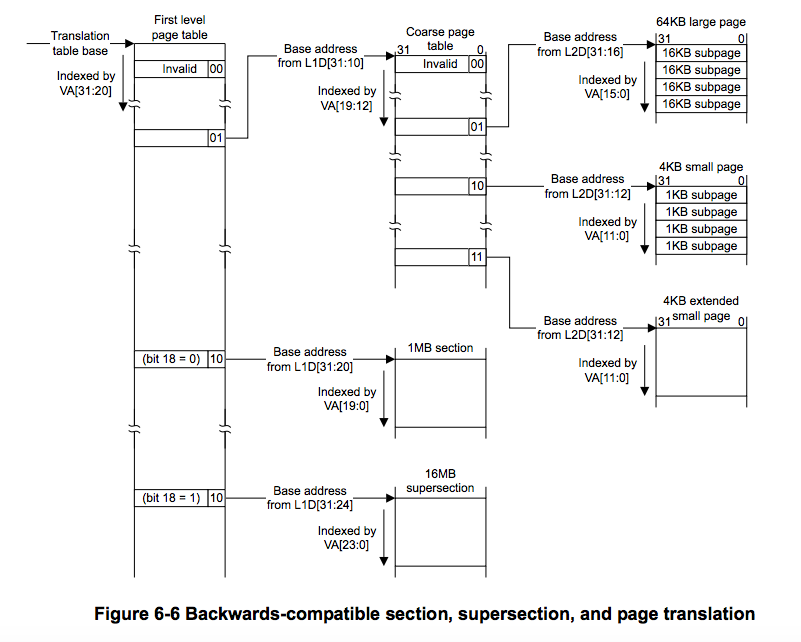
\includegraphics[width=5in]{paging}
			\title{ARM 虚拟地址翻译流程}
		\end{center}
		
		从图中可以看出,ARM的一级页表有4096项,虚拟地址的高12位是一级页表索引,因此一级页表占16KB。
		一级页表项的末两位决定了翻译方式:
		\begin{itemize}
			\item 00: 页表项不存在
			\item 01:指向二级页表,
			\item 10(bit 18 = 0):指向1MB内存页
			\item 10(bit 18 = 1):指向16MB内存页
		\end{itemize}
		因此ARM中可以混合使用一级页表和二级页表。
		二级页表有256项,因此页表占1KB。二级页表项的末两位同样决定了翻译方式:
		\begin{itemize}
			\item 00: 页表项不存在
			\item 01:指向64KB内存页
			\item 1X:指向4KB内存页
		\end{itemize}	
		在我的实现中,混合使用了1MB的页和4KB的页。
		
		entrypgdir.c中定义了启动时加载的页表,与x86实现类似,我们利用一级页表1MB内存页,将[0, 16MB)物理内存同时映射到[0~16MB)和[KERNBASE, KERNBASE + 16MB)
		的虚拟地址上。然后将GPIOBASE起始的1MB内存映射到0x3F200000,用于控制台I/O。更完整的页表将在pmap.c中重新定义。
		\begin{lstlisting}
			pde_t entry_pgdir[NPDENTRIES] __attribute__((aligned(16 * 1024))) = {
				[0x0] = 0x00000002,
				[0x1] = 0x00100002,
				[0x2] = 0x00200002,
				// ........
				[0xf] = 0x00f00002,
				
				[GPIOBASE >> 20] = 0x3f200002,
				
				[0xf00] = 0x00000002,
				[0xf01] = 0x00100002,
				[0xf02] = 0x00200002,
				// .........
				[0xf0f] = 0x00f00002,
			};
		\end{lstlisting}
		
	\subsection{pmap.c}
	在这个文件的移植过程中,我尽量保持了JOS的原貌,接口做到一一对应。
	pmap.c主要实现了三个功能:物理页的管理,页表映射管理,内核页表管理。
	\paragraph{物理页的管理}
	我保持了JOS中原有的数据结构,使用PageInfo数组pages记录每一个物理页的信息,并把空闲物理页用链表存起来方便存取。由于在实现中混用了1MB和4KB页,我使用了一点技巧:将内核栈、启动时页表entry\_pgdir、内核页表kern\_pgdir放入data段,因此它们都在end之下。end是在kernel.ld中定义的,标记着bss段结束。我们直接映射256MB物理内存到KERNBASE以上来管理end以下的数据(data段,bss段),而将其他物理内存分成4KB的页管理。
	pages初始化:
	\begin{lstlisting}
	void page_init(void) {
		extern char end[];
		for (physaddr_t addr = 0; addr < TOTAL_PHYS_MEM; addr += PGSIZE) {
			struct PageInfo *pg = pa2page(addr);
			if (addr == 0 || (0x100000 <= addr && addr < PADDR(end)))
			continue;
			pg->pp_ref = 0;
			pg->pp_link = page_free_list;
			page_free_list = pg;
		}
	}
	\end{lstlisting}
	
	分配一个物理页和删除一个物理页,这两个函数和JOS的实现完全一样,所有移植过程中不需要修改。
	分配一个物理页:
	\begin{lstlisting}
	struct PageInfo * page_alloc(int alloc_flags)
	{
		if (page_free_list == NULL) return NULL;
		struct PageInfo* ret = page_free_list;
		page_free_list = ret->pp_link;
		if (alloc_flags & ALLOC_ZERO) 
		memset(page2kva(ret), 0, PGSIZE);
		ret->pp_link = NULL;
		return ret;
	}
	\end{lstlisting}
	
	
	删除一个物理页:
	\begin{lstlisting}
	void page_free(struct PageInfo *pp)
	{
		if (pp->pp_ref == 0) {
		pp->pp_link = page_free_list;
		page_free_list = pp;
		}
		else {
		panic("pp->pp_ref is not zero. Wrong call of the page_free!!!");
	}
	}
	\end{lstlisting}	
	\paragraph{页表映射管理}
	这个里面涉及了几个函数:pgdir\_walk, boot\_map\_region, page\_insert, page\_lookup, page\_remove。
	这几个函数和JOS on x86的实现上几乎相同,区别在于页表的权限设置上。我将所有的页都分配为domain  0。
	domain 0 就是前面所说的域的概念,一共具有16个域。我把它全部映射成domain 0,就是方便起见,将所有的页都分配给了domain 0。
	
	值得一提的是,由于arm 中二级页表是1KB,而页的大小是4KB,这里,我没有简单的为每个页表都分配一个页,而是实现了一个pgtbl\_alloc()的函数。这个函数的功能是,每次调用都会返回一个空闲的1KB的空间。所以,每调用这个函数4次,他会新申请一个物理页。
	
	
	\begin{lstlisting}
	static pte_t* pgtbl_alloc()
	{
		static pte_t* tbl = NULL;
		if ((uintptr_t)tbl % PGSIZE == 0) {
		struct PageInfo *pg = page_alloc(ALLOC_ZERO);
		if (pg == NULL) return NULL;
		tbl = page2kva(pg);
		pg->pp_ref++;
		}
		pte_t *ret = tbl;
		tbl += NPTENTRIES * 4;
		return ret;
	}
	\end{lstlisting}
	
	JOS on Arm 和JOS on x86还有一点区别在于: x86每页都是4KB,有一个自映射的概念,但是ARM的页的大小不同,所有很难有自映射的概念。所以在部分的实现中,还是有些许区别的。这里实现很简单,就不加赘述了。
	
	\paragraph{内核页表初始化}
	
	我们采用和x86类似的内存布局,首先是将kernel base0xf0000000以上的256MB的空间直接映射成物理地址空间。然后KERNBASE以下依次是内核栈,MMIO, GPIO的内存空间。
	
	我初始化了这些映射,具体详见mem\_init()中的部分代码,同时mem\_init()还装载了Kern\_pgdir到CP15的C2寄存器中,并且使之生效。最后设置了domain 0的状态为client,即需要检查权限位。
	
	\begin{lstlisting}
	void mem_init()
	{
		page_init();
		
		
		// map physical memory
		for (uintptr_t addr = KERNBASE; addr != 0; addr += PTSIZE) {
			kern_pgdir[PDX(addr)] = PADDR((void*)addr) | PDE_ENTRY_1M | PDE_NONE_U;
			kern_pgdir[PDX(PADDR((void*)addr))] = 0;
		}
		
		// map kernel stack
		kern_pgdir[PDX(KSTACKTOP - KSTKSIZE)] = PADDR(bootstack) | PDE_ENTRY_1M | PDE_NONE_U;
		
		// map gpio memory-map
		kern_pgdir[PDX(GPIOBASE)] = 0x3F200000 | PDE_ENTRY_1M | PDE_NONE_U;
		
		
		load_pgdir(PADDR(kern_pgdir));
		set_domain(0, DOMAIN_CLIENT);
		
		check_page_free_list();
		check_page_alloc();
		check_page();
		check_kern_pgdir();
		check_page_installed_pgdir();
	}
		\end{lstlisting}
		
		\begin{lstlisting}
		static void set_domain(int did, int priv) {
			int clear_bit = ~(11 << (2 * did));
			int new_priv = priv << (2 * did);
			asm("mrc p15, 0, r0, c3, c0, 0\n"
			"and r0, r0, %0\n"
			"orr r0, r0, %1\n"
			"mcr p15, 0, r0, c3, c0, 0\n" 
			: 
			: "r"(clear_bit), "r"(new_priv)
			: "r0");
		}
		static inline void load_pgdir(uint32_t value) {
			asm volatile ("mcr p15, 0, %0, c2, c0, 0" : : "r"(value));
		}
		\end{lstlisting}
		
	\subsection{Unchanged Code for Jos on Arm }
	JOS 移植中,基于文件层面的,有一些代码需要修改,有一些代码不需要修改,为了方便查看起见,我将前两个lab移植 对文件的修改部分总结如下:
			
			修改过的文件列表
		文件夹 lib\\
		lib/printfmt.c \\
		lib/readline.c \\
		lib/string.c\\ \\
		文件夹 inc\\
		inc/assert.h\\
		inc/elf.h \\
		inc/error.h\\ 
		inc/stab.h \\
		inc/stdarg.h\\ 
		inc/stdio.h \\
		inc/string.h \\
		inc/types.h \\ \\
		文件夹 kern\\
		kern/kdebug.c \\
		kern/kdebug.h \\
		kern/monitor.h \\
		kern/printf.c\\
		kern/pmap.h\\
		
		
		修改过的文件列表:\\
		inc文件夹\\
		inc/memlayout.h\\
		inc/mmu.h\\ \\
		kern文件夹\\
		kern/entry.S\\
		kern/init.c\\
		kern/console.c\\
		kern/console.h\\
		kern/entrypgdir.c\\
		kern/monitor.c\\
		kern/pmap.c  \\
	
\section{Conclusion}
		
		我完成了所有JOS 的lab1 和lab2 的arm移植,并且通过了所有的check点。
		
		\textbf{lab1}
		
		\begin{itemize}
			\item 成功设置了控制台IO
			\item 成功进入了monitor
			\item 成功使用了Backtrace的控制台命令
		\end{itemize} 	
	
		\textbf{lab2}
		
		\begin{itemize}
			\item check\_page\_free\_list()成功通过测试
			\item 	check\_page\_alloc()成功通过测试
			\item check\_page()成功通过测试
			\item check\_kern\_pgdir()成功通过测试
			\item check\_page\_installed\_pgdir()成功通过测试
		\end{itemize}
		
		注: 这里的check函数均为JOS on x86的修改版,删去了x86体系结构相关的检查,比如自映射的检查,并修改了权限位的检查,改成了arm的相应权限位的检查。

------------------------------------------------

This completes the JOS  on ARM!!!
\end{CJK}
\end{document}
